\subsection{MSVC: x86}

\lstinputlisting{patterns/04_scanf/2_global/ex2_MSVC.asm}

In this case the \TT{x} variable is defined in the \TT{\_DATA} segment and no memory is allocated in the local stack. It is accessed directly, not through the stack. 
Uninitialized global variables take no space in the executable file
(indeed, why one needs to allocate space for variables initially set to zero?), 
but when someone accesses their address, 
the \ac{OS} will allocate a block of zeroes there\footnote{That is how a \ac{VM} behaves}.

Now let's explicitly assign a value to the variable:

\lstinputlisting{patterns/04_scanf/2_global/default_value.c.\LANG}

We got:

\begin{lstlisting}
_DATA	SEGMENT
_x	DD	0aH

...
\end{lstlisting}

Here we see a value \TT{0xA} of DWORD type (DD stands for DWORD = 32 bit) for this variable.

If you open the compiled .exe in \IDA, you can see the \IT{x} variable placed at the beginning of 
the \TT{\_DATA} segment, and after it you can see text strings.

If you open the compiled .exe from the previous example in \IDA, where the value of \IT{x} was not set, you would see something like this:

\begin{lstlisting}
.data:0040FA80 _x              dd ?                    ; DATA XREF: _main+10
.data:0040FA80                                         ; _main+22
.data:0040FA84 dword_40FA84    dd ?                    ; DATA XREF: _memset+1E
.data:0040FA84                                         ; unknown_libname_1+28
.data:0040FA88 dword_40FA88    dd ?                    ; DATA XREF: ___sbh_find_block+5
.data:0040FA88                                         ; ___sbh_free_block+2BC
.data:0040FA8C ; LPVOID lpMem
.data:0040FA8C lpMem           dd ?                    ; DATA XREF: ___sbh_find_block+B
.data:0040FA8C                                         ; ___sbh_free_block+2CA
.data:0040FA90 dword_40FA90    dd ?                    ; DATA XREF: _V6_HeapAlloc+13
.data:0040FA90                                         ; __calloc_impl+72
.data:0040FA94 dword_40FA94    dd ?                    ; DATA XREF: ___sbh_free_block+2FE
\end{lstlisting}

\TT{\_x} is marked with \TT{?} with the rest of the variables that do not need to be initialized. 
This implies that after loading the .exe to the memory, a space for all these variables is to be 
allocated and filled with zeroes \cite[6.7.8p10]{C99TC3}. 
But in the .exe file these uninitialized variables do not occupy anything.
This is convenient for large arrays, for example.

\ifdefined\IncludeOlly
\EN{\clearpage
\subsection{MSVC: x86 + \olly}
\myindex{\olly}

Things are even simpler here:

\begin{figure}[H]
\centering
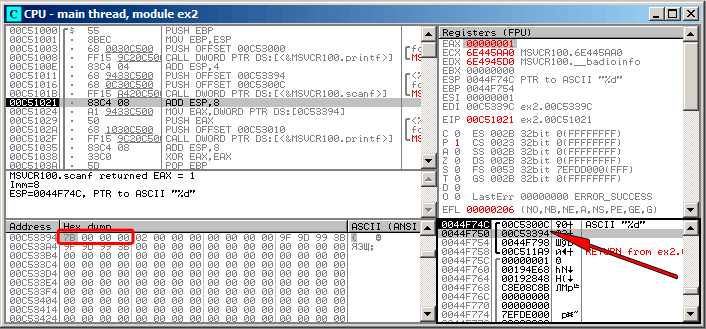
\includegraphics[scale=\FigScale]{patterns/04_scanf/2_global/ex2_olly_1.png}
\caption{\olly: after \scanf execution}
\label{fig:scanf_ex2_olly_1}
\end{figure}

The variable is located in the data segment.
After the \PUSH instruction (pushing the address of $x$) gets executed, 
the address appears in the stack window. Right-click on that row and select \q{Follow in dump}.
The variable will appear in the memory window on the left.
After we have entered 123 in the console, 
\TT{0x7B} appears in the memory window (see the highlighted screenshot regions).

But why is the first byte \TT{7B}?
Thinking logically, \TT{00 00 00 7B} should be
there.
The cause for this is referred as  \gls{endianness}, and x86 uses \IT{little-endian}.
This implies that the lowest byte is written first, and the highest written last.
Read more about it at: \myref{sec:endianness}.
Back to the example, the 32-bit value is loaded from this memory address into \EAX and passed to \printf.

The memory address of $x$ is \TT{0x00C53394}.

\clearpage
In \olly we can review the process memory map (Alt-M)
and we can see that this address is inside the \TT{.data} PE-segment of our program:

\begin{figure}[H]
\centering
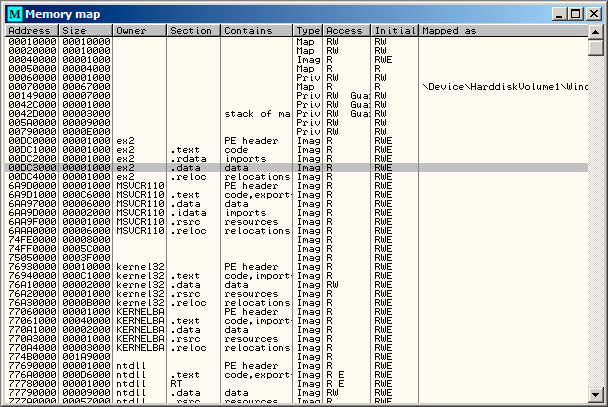
\includegraphics[scale=\FigScale]{patterns/04_scanf/2_global/ex2_olly_2.png}
\caption{\olly: process memory map}
\label{fig:scanf_ex2_olly_2}
\end{figure}

}
\RU{\clearpage
\subsectionold{MSVC: x86 + \olly}
\myindex{\olly}

Тут даже проще:

\begin{figure}[H]
\centering
\myincludegraphics{patterns/04_scanf/2_global/ex2_olly_1.png}
\caption{\olly: после исполнения \scanf}
\label{fig:scanf_ex2_olly_1}
\end{figure}

Переменная хранится в сегменте данных.
Кстати, после исполнения инструкции \PUSH (заталкивающей адрес $x$) адрес появится в стеке, 
и на этом элементе можно нажать правой кнопкой, выбрать \q{Follow in dump}.
И в окне памяти слева появится эта переменная.

После того как в консоли введем 123, здесь появится \TT{0x7B}.

Почему самый первый байт это \TT{7B}?
По логике вещей, здесь должно было бы быть \TT{00 00 00 7B}.
Это называется \gls{endianness}, и в x86 принят формат \IT{little-endian}.
Это означает, что в начале записывается самый младший байт, а заканчивается самым старшим байтом.
Больше об этом: \myref{sec:endianness}.

Позже из этого места в памяти 32-битное значение загружается в \EAX и передается в \printf.

Адрес переменной $x$ в памяти \TT{0x00C53394}.

\clearpage
В \olly{} мы можем посмотреть карту памяти процесса (Alt-M) и увидим, что этот адрес
внутри PE-сегмента \TT{.data} нашей программы:

\begin{figure}[H]
\centering
\myincludegraphics{patterns/04_scanf/2_global/ex2_olly_2.png}
\caption{\olly: карта памяти процесса}
\label{fig:scanf_ex2_olly_2}
\end{figure}
}
\ITA{\clearpage
\subsectionold{MSVC: x86 + \olly}
\myindex{\olly}

Il quadro qui è ancora più semplice:

\begin{figure}[H]
\centering
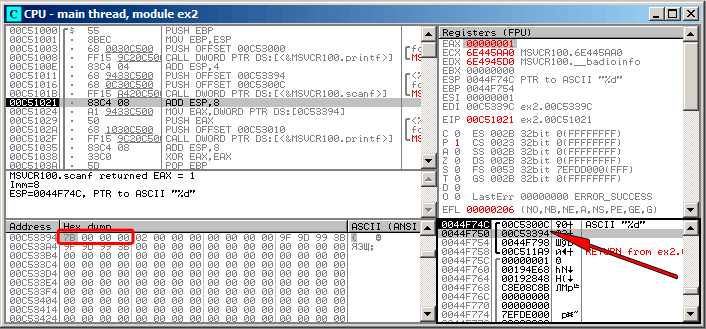
\includegraphics[scale=\FigScale]{patterns/04_scanf/2_global/ex2_olly_1.png}
\caption{\olly: after \scanf execution}
\label{fig:scanf_ex2_olly_1}
\end{figure}

La variabile è collocata nel data segment.
Dopo che l'istruzione \PUSH (che fa il push dell'indirizzo di $x$) viene eseguita, 
l'indirizzo appare nella finestra dello stack. Facciamo click destro su quella riga e selezioniamo \q{Follow in dump}.
La variabile apparirà nella finestra di memoria a sinistra.
Dopo aver inserito il valore 123 in console, 
\TT{0x7B} apparirà nella finestra della memoria (vedere regioni evidenziate nello screenshot).

Ma perchè il primo byte è \TT{7B}?
A rigor di logica, dovremmo trovare \TT{00 00 00 7B}.
La causa per cui troviamo invece \TT{7B} è detta \gls{endianness}, e x86 usa la convenzione \IT{little-endian}.
Ciò significa che il byte piu basso è scritto per primo, e quello più alto per ultimo.
Maggiori informazioni sono disponibili nella sezione: \myref{sec:endianness}.
Tornando all'esempio, il valore a 32-bit è caricato da questo indirizzo di memoria in \EAX e passato a \printf.

L'indirizzo in memoria di $x$ è \TT{0x00C53394}.

\clearpage
In \olly possiamo osservare la mappa di memoria di un processo  (process memory map, Alt-M)
e notare che questo indirizzo è dentro il segmento PE \TT{.data} del nostro programma:

\begin{figure}[H]
\centering
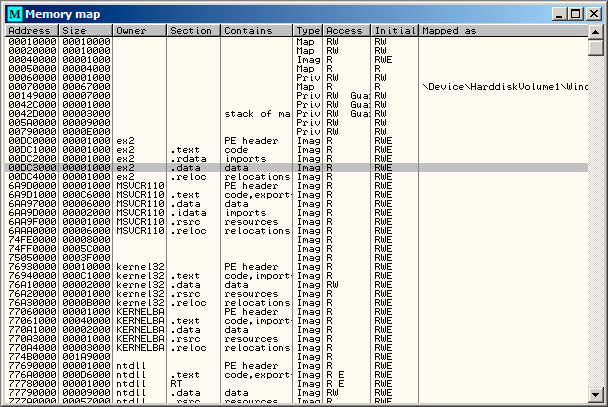
\includegraphics[scale=\FigScale]{patterns/04_scanf/2_global/ex2_olly_2.png}
\caption{\olly: process memory map}
\label{fig:scanf_ex2_olly_2}
\end{figure}

}

\fi

\ifdefined\IncludeGCC
\subsection{GCC: x86}

\myindex{ELF}
The picture in Linux is near the same, with the difference that the uninitialized variables are located in the \TT{\_bss} segment. 
In \ac{ELF} file this segment has the following attributes:

\begin{lstlisting}
; Segment type: Uninitialized
; Segment permissions: Read/Write
\end{lstlisting}

If you, however, initialise the variable with some value e.g. 10, 
it is to be placed in the \TT{\_data} segment, which has the following attributes:

\begin{lstlisting}
; Segment type: Pure data
; Segment permissions: Read/Write
\end{lstlisting}
\fi

\subsection{MSVC: x64}

\lstinputlisting[caption=MSVC 2012 x64]{patterns/04_scanf/2_global/ex2_MSVC_x64.asm.\LANG}

The code is almost the same as in x86.
Please note that the address of the $x$ variable is passed to \TT{scanf()} using a \LEA instruction,
while the variable's value is passed to the second \printf using a \MOV instruction.
\TT{DWORD PTR}---is a part of the assembly language (no relation to the machine code),
indicating that the variable data size is 32-bit and the \MOV instruction has to be encoded accordingly.

